\documentclass[../main.tex]{subfiles}
\graphicspath{{\subfix{../images/}}}
\begin{document}
\section*{Term 1 Week 7}
\begin{enumerate}
    \item 
    Combine the two equations to eliminate the \(xy\) term.\\
    $
    \!
    \begin{aligned}[t]
        2.5x^2+5xy+7.5y^2
        &=5\\
        +3x^2-5xy+7y^2
        &=15\\ 
        5.5x^2+14.5y^2
        &=20\\
        11x^2+29y^2
        &=40\\
        x^2
        &=\frac{40-29y^2}{11}\\
    \end{aligned}
    $
    
    Substitute this into one of the equations:\\
    \(\frac{40-29y^2}{11}+2y\sqrt{\frac{40-29y^2}{11}}+3y^2=2\)\\

    \(\frac{4y^2}{11}+2y\sqrt{\frac{40-29y^2}{11}}=-\frac{18}{11}\)\\

    \(2y\sqrt{\frac{40-29y^2}{11}}=-\frac{18-4y^2}{11}\)\\

    \(4y^2(\frac{40-29y^2}{11})=\frac{324+144y^2+16y^4}{121}\)\\

    \(\frac{160y^2}{11}-\frac{116y^4}{11}=\frac{324+144y^2+16y^4}{121}\)\\

    \(1760y^2-1276y^4=324+144y^2+16y^4\)\\

    \(1292y^4-1616y^2+324=0\)\\

    Substitute \(u=y^2\) and solve:\\
    \(1292u^2-1616u+324=0\)\\
    \(u=1, \frac{81}{323}\)\\

    \(y^2=1\)\\
    \(y=\pm 1\)\\
    Substitute into x formula to get x-coordinates:\\
    \(x=\pm \sqrt{\frac{40-29(1)^2}{11}}=\pm 1\)\\

    So possible coordinates are:\\
    \((1,1), (1, -1), (-1, 1), (-1,-1)\)\\

    \(y^2=\frac{81}{323}\)\\
    \(y=\pm \sqrt{\frac{81}{323}}\)\\
    Substitute to get x-coordinates:\\
    \(x=\pm \sqrt{\frac{40-29(\frac{81}{323})}{11}}\)\\

    So possible coordinates are:\\
    \((\sqrt{\frac{961}{323}}, \sqrt{\frac{81}{323}}), (\sqrt{\frac{961}{323}},-\sqrt{\frac{81}{323}}), (-\sqrt{\frac{961}{323}}, \sqrt{\frac{81}{323}}), (-\sqrt{\frac{961}{323}}, -\sqrt{\frac{81}{323}})\)\\

    We need to check that these are valid as by squaring the equation we may have introduced new solutions. Substitute these into one of the original equations to see if they balance.\\
    Turns out the only valid ones are:\\
    \((-1,1), (1, -1), (-\sqrt{\frac{961}{323}}, \sqrt{\frac{81}{323}}), (\sqrt{\frac{961}{323}}, -\sqrt{\frac{81}{323}})\)\\

    NB: Could also be written \((-1,1),(1,-1),(-1.72,0.5008),(1.72,-0.5008)\)
    \begin{figure}[H]
        \centering
        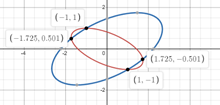
\includegraphics{images/t1w7q1_a.png}
    \end{figure}
    
    \item 
    To minimise \(e^x\) we need to make the exponent as small as possible.\\
    This involves making the square root as large as possible so that we are taking a large number away from 5.\\
    To make the square root as large as possible we need the fraction inside it to be as large as possible. This requires making the denominator as small as we can.\\
    Therefore, we need to minimise the function \(x^2+2x+2\).\\
    Differentiating, we get: \(f'(x)=2x+2 \)\\
    
    To find the minimum, we make it equal to zero and solve:\\
    \(2x+2=0\\
    x=-1\)\\
    
    Therefore, the original function is minimised when x = 1.\\
    \[y=e^{(5-\sqrt{\frac{1}{1^2+2(1)+2}})}=e^4\]\\

    \item 
    Take tan of both sides:\\
    \(\tan(tan^{-1}(x)+\tan^{-1}(2x))=\tan(\frac{\pi}{4})\)\\

    Using the compound angle rule for tan:\\
    
    \(\frac{\tan(\tan^{-1}(x))+\tan(\tan^{-1}(2x))}{1-\tan(\tan^-1(x))\tan(\tan^-1(2x))}=1\)\\

    Since \(\tan\) and \(\tan^{-1}\) are inverse functions, \(\tan(\tan^{-1}(x))=x\)\\

    Giving us:\\
    \(\frac{x+2x}{1-x\times 2x}=1\)\\

    \(\frac{3x}{1-2x^2}=1\)\\

    \(3x=1-2x^2\)\\

    \(2x^2+3x-1=0\)\\

    \(x=0.28, 1.78\) (2 dp)
    
    
\end{enumerate}

\end{document}